%!TEX root = ../../master.tex
\section{Defining Cloud Computing}
Cloud computing represents a paradigm shift in how applications are run and managed. Sosinsky describes the paradigm shift as: \textit{"Cloud computing makes the long-held dream of utility computing possible with a pay-as-you-go, infinitely scalable, universally available system"} \cite[p. 3]{sosinsky2011cloud}. The National Institute of Standards and Technology (NIST) defines cloud computing as: 

\begin{definition}[Definition]
    \textit{"Cloud computing is a model for enabling ubiquitous, convenient, on-demand network access to a shared pool of configurable computing resources (e.g., networks, servers, storage, applications, and services) that can be rapidly provisioned and released with minimal management effort or service provider interaction"} \cite[p. 2]{nist2011definition}
\end{definition}

\noindent 
Cloud computing is distinguished from other types of computing by the notion that resources are virtual and (almost) limitless. The underlying details of the physical systems on which the software runs are abstracted from the perspective of the user. According to Sosinsky the two essential concepts in cloud computing are:

\begin{definition} [Abstraction]
Cloud computing abstracts the details of system implementation from users and developers. Applications run on physical systems that aren't specified, data is stored in locations that are unknown, administration of systems is outsourced to others, and access by users is ubiquitous. \cite[p. 4]{sosinsky2011cloud}    
\end{definition}

\begin{definition} [Virtualization]
Cloud computing virtualizes systems by pooling and sharing resources. Systems and storage can be provisioned as needed from a centralized infrastructure, cost are assessed on a metered basis, multi-tenancy is enabled, and resources are scalable with agility. \cite[p. 4]{sosinsky2011cloud}    
\end{definition}

\noindent
According to NIST, cloud computing can be divided into two distinct sets of models \cite[p. 2-3]{nist2011definition}:
\begin{itemize}
    \item \textbf{Deployment models:} The location and management of the cloud's infrastructure. 
        \begin{itemize}
            \setlength\itemsep{0.05em}
            \vspace{-3mm}
            \item \textit{Public clouds} The cloud infrastructure is for open use by the general public and exists on the premises of the cloud provider.
            \item \textit{Private clouds} The cloud infrastructure is provisioned for exclusive use for a single organization and may exist on or off premises.
            \item \textit{Hybrid cloud} The cloud infrastructure is a composition of two or more deployment models.
            \item \textit{Community cloud} The cloud infrastructure is provisioned for exclusive use by a specific community and may exist on or off premises.
        \end{itemize}
    \item \textbf{Service models:} The types of services accessible on a cloud computing platform.
        \begin{itemize}
            \setlength\itemsep{0.05em}
            \vspace{-3mm}
            \item \textit{Infrastructure as a Service} (IaaS): The cloud provider manages the virtualization layer and below (Figure~\ref{fig:cloud_stack}). You manage from the OS layer and above.
            \item \textit{Platform as a Service} (PaaS): The cloud provider manages the runtime layer and below (Figure~\ref{fig:cloud_stack}). You manage from the data/application layer.
            \item \textit{Software as a Service} (SaaS): The cloud provider manages the complete operating environment with applications, management, and a user interface (Figure~\ref{fig:cloud_stack}).
        \end{itemize}
\end{itemize} 

\noindent
The cloud stack (Figure~\ref{fig:cloud_stack}) is comprised of several enabling technologies that can be combined in various ways. As previously mentioned, virtualization has played an important role in the software stack.

\begin{figure}[H]
  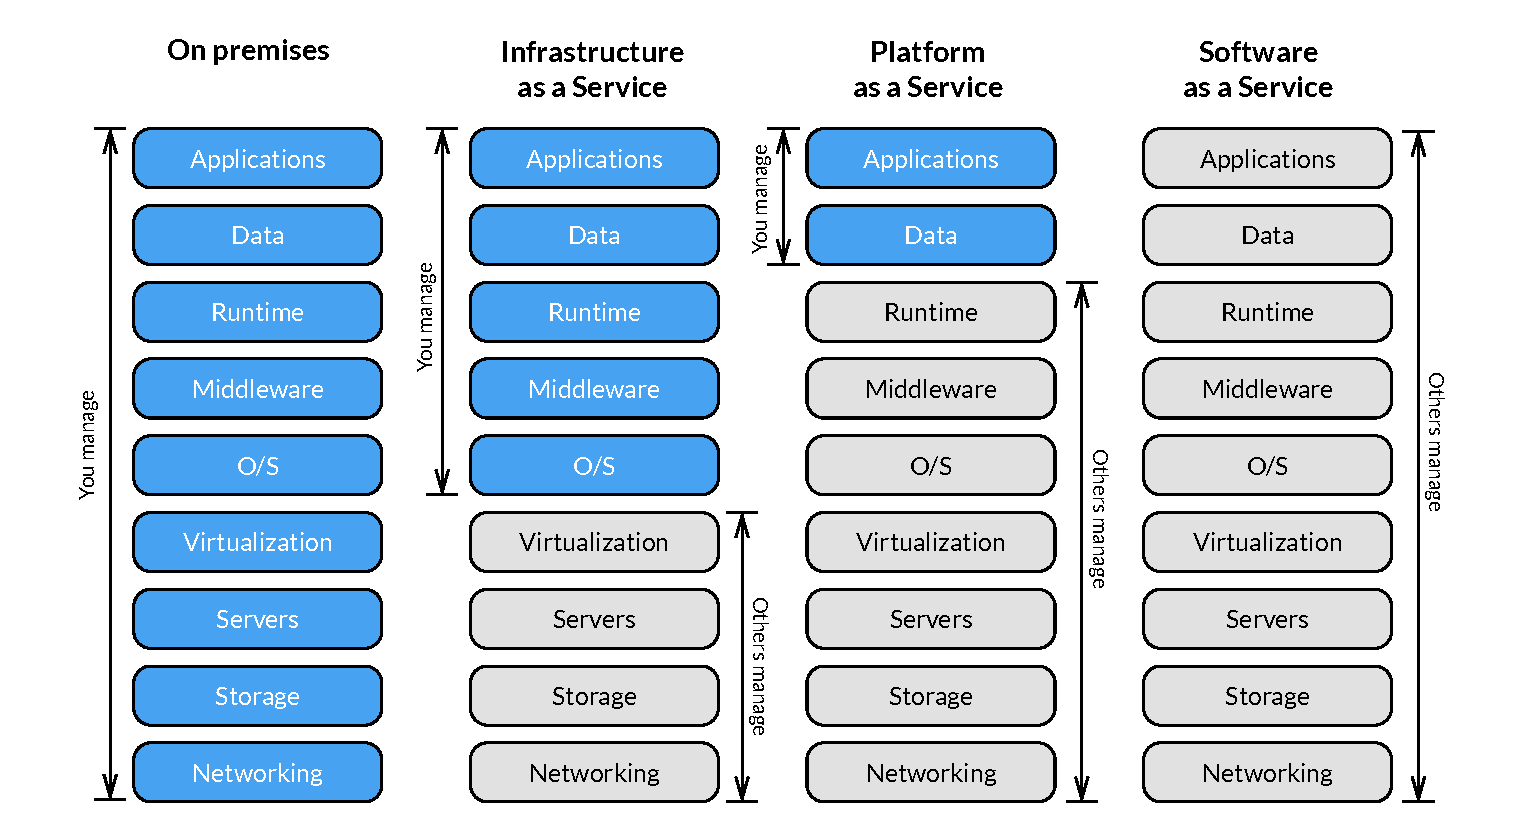
\includegraphics[scale=0.55]{figures/cloud_stack}
  \caption{Cloud Stack and Deployment Models}
\end{figure}
\label{fig:cloud_stack}

\noindent
Google has challenged NIST's definition of service models by introducing the concept of Container as a Service (CaaS). Burns et al describe this new service model: \textit{"Containers encapsulates the application environment abstracting away many details of machines and operating systems from the application developer and the deployment infrastructure"} \cite[p. 74]{burns2016borg_omega_kubernetes}. By this definition, Container as a Service is placed between Infrastructure as a Service and Platform as a Service. Containerization will be discussed later in this chapter. \\

\noindent
NIST describes some of the essential characteristics of cloud computing as: on-demand self-service, broad network access, resource pooling, rapid elasticity, and measured service \cite[p. 2]{nist2011definition}. Sosinsky describes additional advantages being: lower costs, ease of utilization, quality of service, reliability, outsourced IT management, simplified maintenance and upgrade, and low barrier to entry \cite[p.17-18]{sosinsky2011cloud}. 
An example of the elasticity in cloud computing is coping with the additional traffic on Black Friday. If a retailer is required to run the hardware needed for Black Friday peak hours, much energy would be wasted the rest of the year. Companies have different peak hours, and by utilizing the elasticity of cloud computing, it becomes possible to scale resources up and down dynamically. \\

\noindent
Among the disadvantages of cloud computing are: less customizability, latency, privacy, and security. \\

\noindent
An often used analogy is that computational power from cloud computing corresponds to electricity from the power grid. This illustrates the benefit of the pay-as-you-go model instead of everyone acquiring a power plant. It is, though, important to note that you trust a cloud vendor with your data, as pointed out by Subramanian \cite{subramanian2010electricity_metaphor}. This also justifies the hybrid cloud model in which you keep some of the hardware under your own control e.g. for personal data.


